% Template for ICIP-2014 paper; to be used with:
%          spconf.sty  - ICASSP/ICIP LaTeX style file, and
%          IEEEbib.bst - IEEE bibliography style file.
% --------------------------------------------------------------------------
\documentclass{article}
\usepackage{spconf,amsmath,graphicx}
\usepackage{subfig}
% Example definitions.
% --------------------
\def\x{{\mathbf x}}
\def\L{{\cal L}}

% Title.
% ------
%\title{AUTHOR GUIDELINES FOR ICIP 2014 PROCEEDINGS MANUSCRIPTS}
%\title{Image Denoising with Fast Mixed-–band Wavelet Transform on the GPU}
\title{Fast 3D Mixed-band Wavelet Transform on the GPUs and Compressive Sensing Reconstruction on 3D Volume of MRI}
%
% Single address.
% ---------------
\name
{
	Tran~Minh~Quan and~Won-Ki~Jeong, Member, IEEE % <-this % stops a space
}
\address{Ulsan National Institute of Science and Technology, 
School of Electrical and Computer Engineering, \\
UNIST-gil 50 (100 Banyeon-ri), Eonyang-eup, Ulju-gun, Ulsan, South Korea, 689-798}

%\thanks{T.M. Quan, and W-K. Jeong are with Ulsan National Institute of Science and Technology, Ulsan, South Korea.}
%\name{Author(s) Name(s)\thanks{Thanks to XYZ agency for funding.}}
%\address{Author Affiliation(s)}
%
% For example:
% ------------
%\address{School\\
%	Department\\
%	Address}
%
% Two addresses (uncomment and modify for two-address case).
% ----------------------------------------------------------
%\twoauthors
%  {A. Author-one, B. Author-two\sthanks{Thanks to XYZ agency for funding.}}
%	{School A-B\\
%	Department A-B\\
%	Address A-B}
%  {C. Author-three, D. Author-four\sthanks{The fourth author performed the work
%	while at ...}}
%	{School C-D\\
%	Department C-D\\
%	Address C-D}
%
\begin{document}
%\ninept
%
\maketitle
\begin{abstract}
%% proposal_main.tex

Serving the most basic building block in the JPEG2000 compression pipeline~\cite{skodras_jpeg_2001}, discrete wavelet transform (DWT) is well-known for sparsifying the signal. 
Traditional DWT comprises many steps including: downsampling, filtering and moving the pixels of the result image to separate wavelet sub-bands. 
Later, the lifting-scheme technique comes up to increase performance of DWT on the CPU side. 
It divides the filter scheme into intermediate stages and leverages the implicit parallelism. 
By recognizing the main bottleneck of DWT comes from non-contiguous memory accessing and frequency coefficients moving, mixed-band algorithm attempts to store the sub-band of wavelet decomposition in the interleave positions and utilize the fast-on-chip GPU memories (e.g. shared memory) to process multi-level wavelet decomposition.
Taking into account with the advantages of this feature, we fulfill the picture in which the quality of Compressive Sensing Reconstruction on 3D MRI can be enhanced and the entire process can be speed up by using 3D mixed-band Wavelet Transform on GPU.

% the mixed-band wavelet algorithm on the GPUs. 
% By recognizing the main bottleneck of DWT comes from uncoaslesced memory accessing and frequency coefficients moving, mixed-band algorithm attempts to store the sub-band of wavelet decomposition in the interleave positions and utilize the fast-on-chip GPU memories (e.g. shared memory) to conduct arithmetic operations for multi-level wavelet computing. %The proposed method is well-fit to the multi-dimension wavelet and is the promising application for bio-medical image processing (e.g. CT, MRI, PET, etc.) while we want to deal with very large-scale data which come continuously from the medical scanners or equipments and performing many iterations in some optimization approaches (e.g. Compressive Sensing, Gradient Descent, e.g.).
\end{abstract}
%
\begin{keywords}
Mixed-band, Wavelet, Denoising, CUDA, GPU, Parallel Computing, Compressive Sensing, MRI.
\end{keywords}

\section{Introduction}
\label{intro}
% Describe mixedband
In term of compressibility,  people attempt to downsample the signals (e.g., audio waveform, images, etc.) and filter them with a complement of low- and high-pass filters to compact the information into a sparse representation. 
The new low coefficients form another level of detail of that image. 
Hence, successively processing this one until we reach the final delineation will establish a structure of multi-resolution analysis of signals. 
Fig.~\ref{fig:barbara_tradition} shows a grayscale image and one-, two-, three-level of wavelet decomposition using the simplest filters: Haar family. 
The wavelet coefficients have been mapped onto jet color space which indicates the low value coefficients are blue and the high ones are red. 
If the image has been altered by some noise-like impacts, it will result in the high band of wavelet coefficients contain more non-zero values.



\begin{figure}[t]
	\centering  
	%%%%%%%%%%%%%%%%%%%%%%%%%%%%%%%%%%%%%%%%%%%%%%%%%%%%%%%%%%%%%%%%%%%%%%%
	\subfloat[]
    {  
  		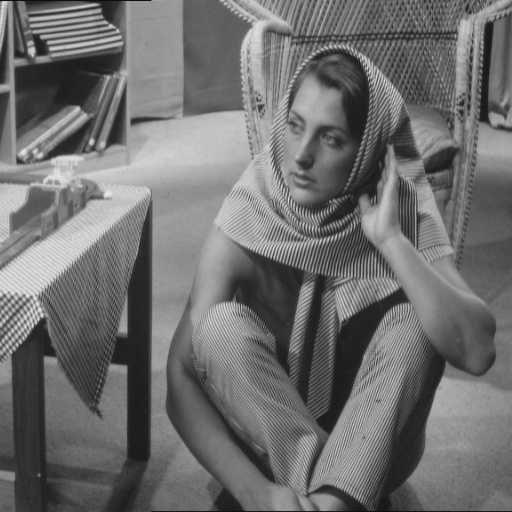
\includegraphics[width=0.3\linewidth]{fig/barbara_gray.png}
	}	\\
    \subfloat[]
    {
		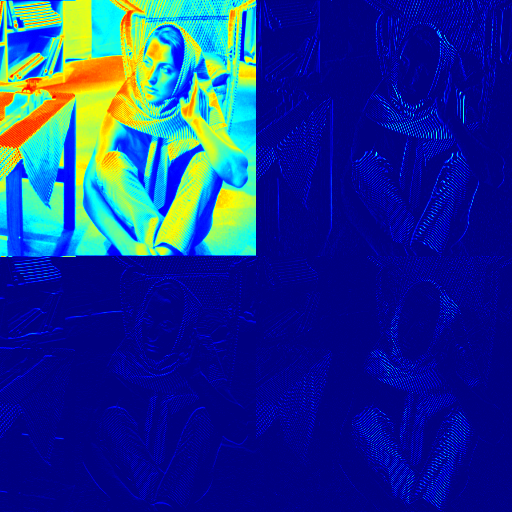
\includegraphics[width=0.3\linewidth]{fig/barbara_tradition_1.png}
    }	
	\subfloat[]
    {  
  		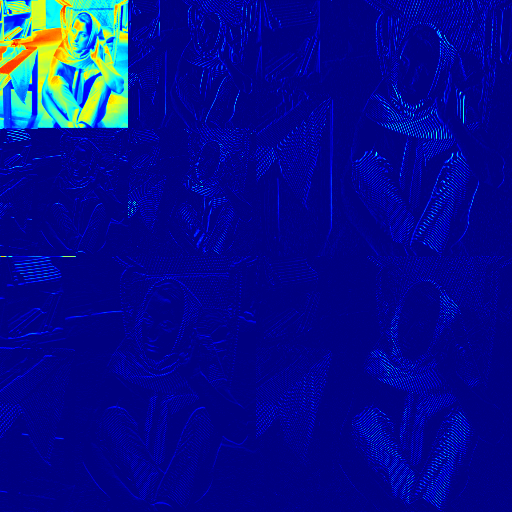
\includegraphics[width=0.3\linewidth]{fig/barbara_tradition_2.png}
	}	
		\subfloat[]
    {  
  		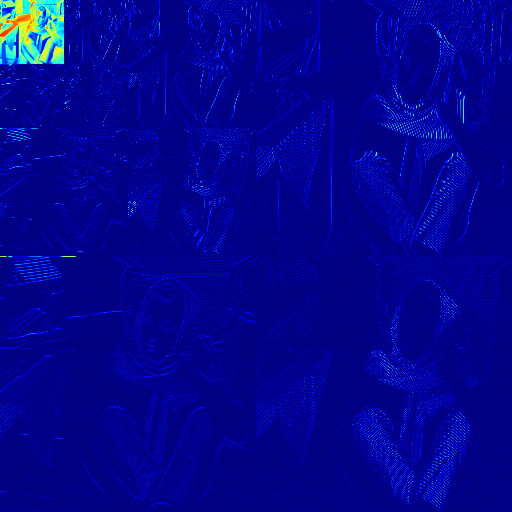
\includegraphics[width=0.3\linewidth]{fig/barbara_tradition_3.png}
	}	\\
\caption{TODO}
\label{fig:barbara_tradition}
\end{figure}



% Describe usefulness
In this paper, we describe straightforward techniques to speedup DWT on the GPU. 
It can be further extended to be embedded into other methods such as combining with Split-Bregman algorithm~\cite{goldstein_split_2009} in 3D Compressive Sensing (CS) MRI  reconstruction, performing many-step image reconstruction by iteratively solving an inverse problem and so on. 
Without going deeply into those mentioned approaches, we bring several advantage features that mixed-band wavelet can be more useful.

% Structure of the paper
The rest of the paper is organized as follows. First, we briefly explain the historical directions of signal analysis as well as data compression and the current state of discrete wavelet transform on this domain in the next.
Second, we describe several ways to deal with the advantages which mixed-band wavelet brings back and how to implement those on the GPU with Compute Unified Device Architecture (CUDA)~\cite{CUDA} programming model.
Third, the performance of traditional wavelet and mixed-band wavelet transform are also measured on either CPU or GPU side to see how benefit we can gain by interleaving wavelet bands on the memory layout.
We also discuss the roll of DWT in 3D CSMRI reconstruction to exploit the  
We conclude our work in the last section, discuss pros and cons and then further suggest some future works in this direction.



\section{Related Work}
\label{relatedwork}
\subsection{Discrete Wavelet Transform}
% 
Conventionally, discrete wavelet transform attempts to decompose an image into two sub-regions: the upper-left stores the low frequency coefficients and the rest stores the high coefficients.
The main bottlenecks of this scheme are memory-bound issues when we have to either access non-contiguous memory or use image transposition. 
Although, the sliding window method can help us to quickly process the image without transposition, we still need to rearrange the coefficients after each filtering step. 
Using the mixed-band algorithm, we can achieve the higher performance of DWT by shuffling the wavelet spectrum and improve the contiguous memory access. 
It also fits elegantly to the GPU programming model. 

\begin{figure}[t]
	\centering  
	%%%%%%%%%%%%%%%%%%%%%%%%%%%%%%%%%%%%%%%%%%%%%%%%%%%%%%%%%%%%%%%%%%%%%%%
	\subfloat[]
    {  
  		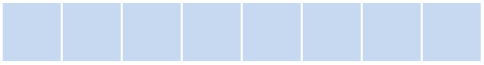
\includegraphics[width=0.3\linewidth]{fig/traditional1d0.png}
	}	\\
    \subfloat[]
    {
		
\includegraphics[width=0.3\linewidth]{fig/traditional1d1.png}
    }	
	\subfloat[]
    {  
  		
\includegraphics[width=0.3\linewidth]{fig/traditional1d2.png}
	}	
		\subfloat[]
    {  
  		
\includegraphics[width=0.3\linewidth]{fig/traditional1d3.png}
	}	\\
	\subfloat[]
    {
		
\includegraphics[width=0.3\linewidth]{fig/mixedband1d1.png}
    }	
	\subfloat[]
    {  
  		
\includegraphics[width=0.3\linewidth]{fig/mixedband1d2.png}
	}	
		\subfloat[]
    {  
  		
\includegraphics[width=0.3\linewidth]{fig/mixedband1d3.png}
	}	\\
	%%%%%%%%%%%%%%%%%%%%%%%%%%%%%%%%%%%%%%%%%%%%%%%%%%%%%%%%%%%%%%%%%%%%%%%
	\subfloat[]
	{  
		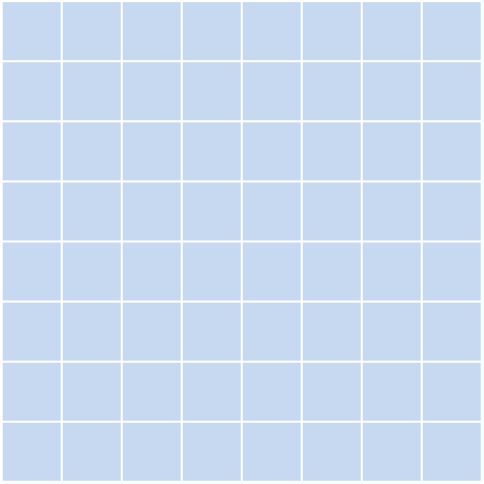
\includegraphics[width=0.3\linewidth]{fig/traditional2d0.png}
	}	\\
	\subfloat[]
	{
		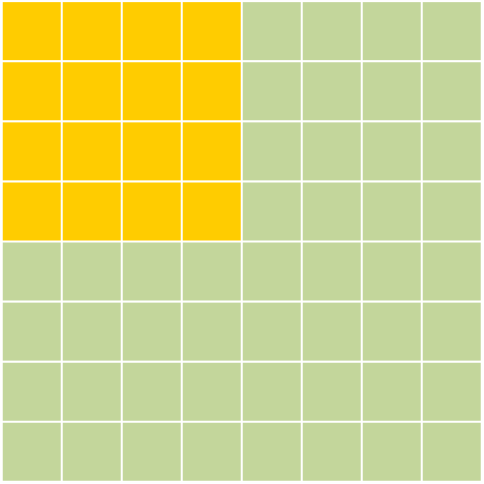
\includegraphics[width=0.3\linewidth]{fig/traditional2d1.png}
	}	
	\subfloat[]
	{  
		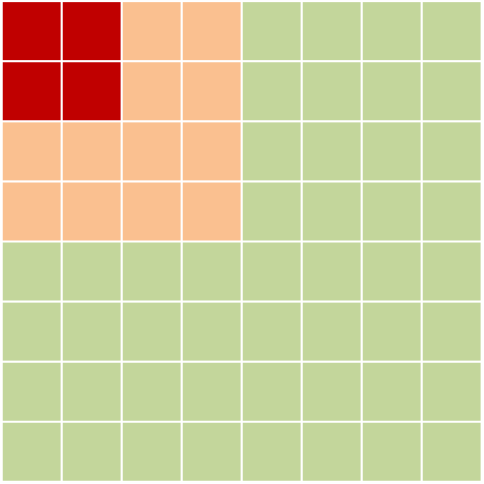
\includegraphics[width=0.3\linewidth]{fig/traditional2d2.png}
	}	
		\subfloat[]
	{  
		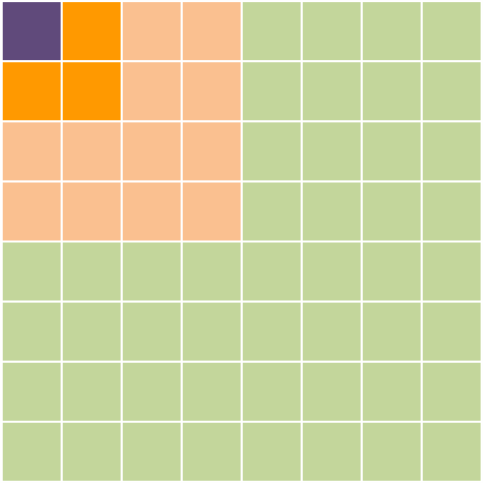
\includegraphics[width=0.3\linewidth]{fig/traditional2d3.png}
	}	\\
	\subfloat[]
	{
		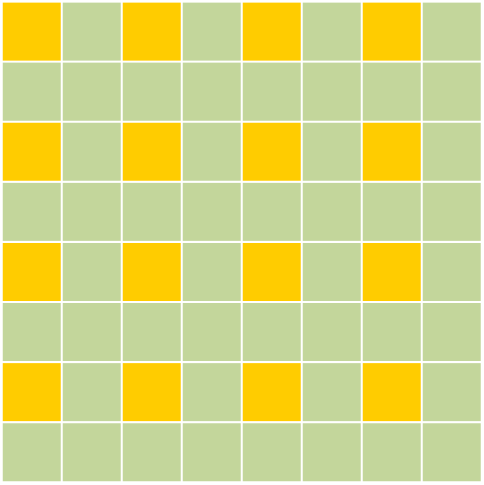
\includegraphics[width=0.3\linewidth]{fig/mixedband2d1.png}
	}	
	\subfloat[]
	{  
		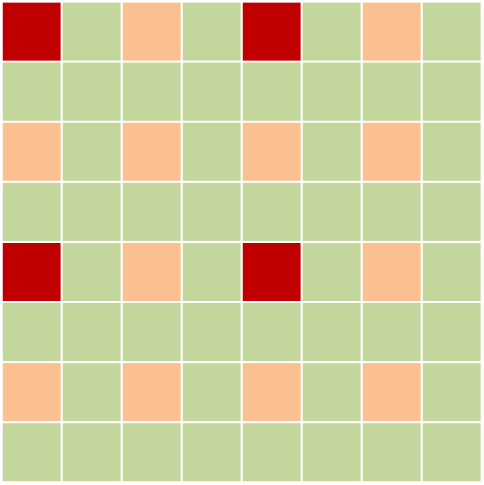
\includegraphics[width=0.3\linewidth]{fig/mixedband2d2.png}
	}	
		\subfloat[]
	{  
		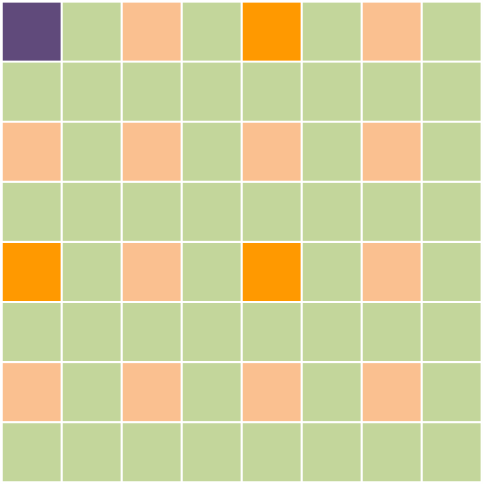
\includegraphics[width=0.3\linewidth]{fig/mixedband2d3.png}
	}	\\
	%%%%%%%%%%%%%%%%%%%%%%%%%%%%%%%%%%%%%%%%%%%%%%%%%%%%%%%%%%%%%%%%%%%%%%%
	\subfloat[]
	{  
		
\includegraphics[width=0.3\linewidth]{fig/traditional3d0.png}
	}	\\
	\subfloat[]
	{
		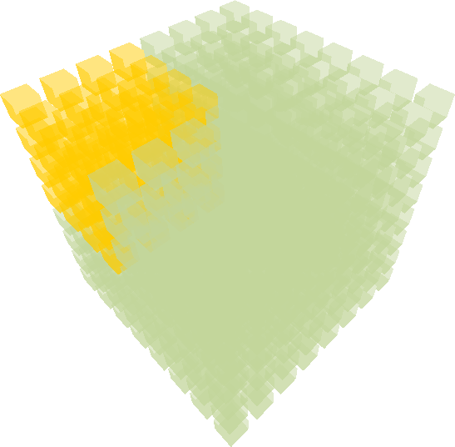
\includegraphics[width=0.3\linewidth]{fig/traditional3d1.png}
	}	
	\subfloat[]
	{  
		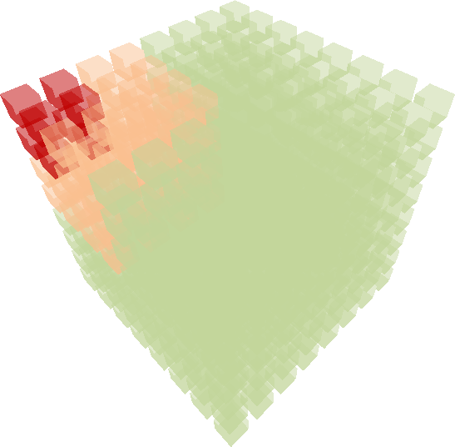
\includegraphics[width=0.3\linewidth]{fig/traditional3d2.png}
	}	
		\subfloat[]
	{  
		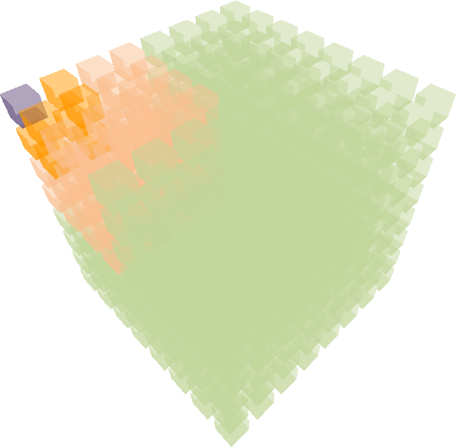
\includegraphics[width=0.3\linewidth]{fig/traditional3d3.png}
	}	\\
	\subfloat[]
	{
		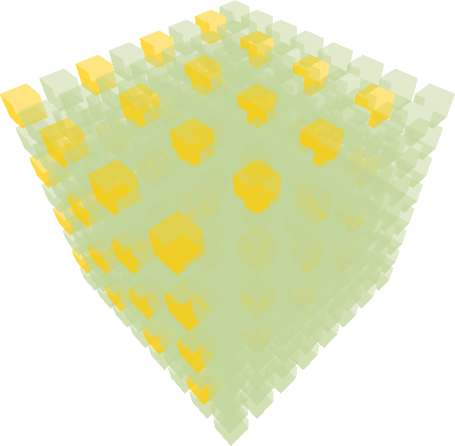
\includegraphics[width=0.3\linewidth]{fig/mixedband3d1.png}
	}	
	\subfloat[]
	{  
		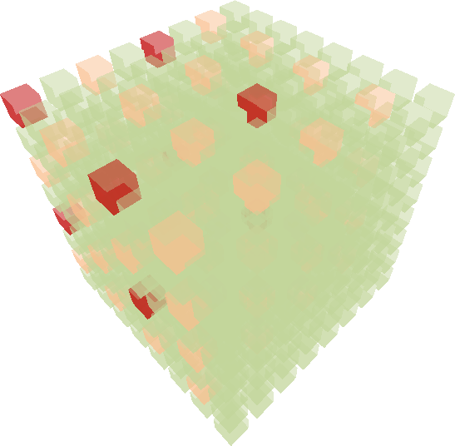
\includegraphics[width=0.3\linewidth]{fig/mixedband3d2.png}
	}	
		\subfloat[]
	{  
		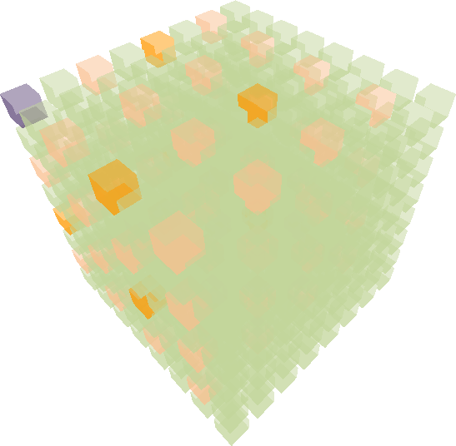
\includegraphics[width=0.3\linewidth]{fig/mixedband3d3.png}
	}	\\
\caption{TODO}
\label{fig:}
\end{figure}

\subsection{Image Denoising with filtering}
\subsection{Image Denoising with DWT and thresholding}
\subsection{Image Denoising with GPU and NVIDIA CUDA}

\section{Method}
\label{method}


\subsection{Parallelize rectilinear lossless wavelet transform}
\subsubsection{Single core CPU implementation}
We attempt to implement a single core CPU version of 2D DWT to have a ground truth for performance comparison with other famous libraries we mentioned above and our next parallel version on the GPU.

Firstly, let us explain the insight of lifting scheme version of 2 types of biorthogonal wavelet families we will deal with: Haar and CDF5/3~\cite{daubechies1992ten}.

\subsubsection{Multi core GPU implementation with filter scheme}
\subsubsection{Multi core GPU implementation with lifting scheme}


%%
\subsection{Perform a one-step self-localization of wavelet coefficients in mixed-band wavelet domain}
\label{subsec:onestepfilter}
The noisy image is firstly transformed to a wavelet domain using lossless biorthogonal wavelet families such as Haar or CDF5/3~\cite{daubechies1992ten}
\subsubsection{Using a mean filter}
\subsubsection{Using a median filter}
\subsubsection{Using a Gaussian filter}
\subsubsection{Using a bilateral filter}

% \subsection{Extend to 3D MRI denoising}
% 3D images acquired from an MRI scanner also contain noise-like impacts (see Fig.~\ref{fig:3dmri}) which come from the high-damped vibrations of signals due to the affects from electro-magnetic waves to water molecules. 
% To reduce such that effects, people employ the smoothing metrics by introducing total variation regularizers into an energy function that they attempt to minimize and iteratively threshold the intermediate results.
% \begin{figure}[t]
	% \centering  
	%%%%%%%%%%%%%%%%%%%%%%%%%%%%%%%%%%%%%%%%%%%%%%%%%%%%%%%%%%%%%%%%%%%%%%
	% \subfloat[]
    % {  
  		% 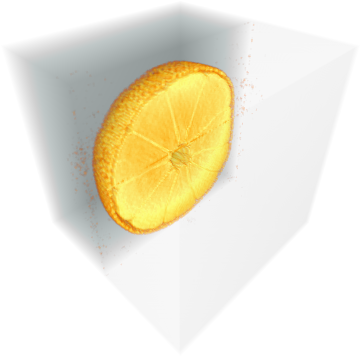
\includegraphics[width=0.5\linewidth]{fig/tangerine128_crop.png}
	% }	
    % \subfloat[]
    % {
		% 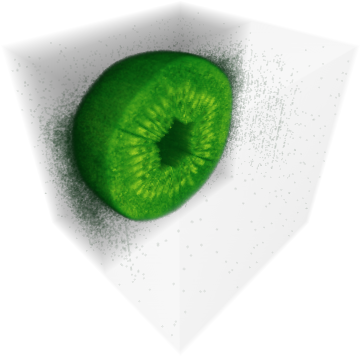
\includegraphics[width=0.5\linewidth]{fig/kiwi128_crop.png}
    % }	
% \caption{TODO}
% \label{fig:3dmri}
% \end{figure}

\subsection{Extend to 3D CSMRI Reconstruction}
In brief, the data come from MRI modality is so-called k-space which represents the samples of the spectrum of the images. 
To get the actual images we want to look at, an inverse Fourier transform is necessary to apply. 
Usually, the scanning procedure requires a long period to obtain the k-space and sometimes cause the danger to such an emergency situation. 
One way to circumvent this case is to discard randomly most of the k-space. 
But if we do not introduce some constraints (e.g, images are sparse in some domain, smoothness and so on) and directly perform inverse Fourier transform to those data, we will receive corruptions in images.
On the other hands, iteratively minimizing a defined energy function with above constraint is a time-consuming task with one single core.
It leads to using a parallel architecture like multi-core CPU or GPU to solve those such computational demand problems. 
To more precise, wavelet can be treated as an operator to establish a regularizer. And instead of perform hard- or soft-thresholding as in~\cite{donoho_-noising_1995}, we will apply the approaches have been mentioned in ~\ref{subsec:onestepfilter}


\section{Results}
\label{results}
\subsection{Compare mixed-band wavelet performance}
\subsubsection{Single core CPU implementation}
We attempt to compare our single core CPU implementation with two other well-known libraries: the Wavelet Package used in CSMRI reconstruction from~\cite{lustig_compressed_2008}  and GNU Scientific Libraries~\cite{GSL}
\subsubsection{GPU implementation}
We also compare with the most recent optimized 2D DWT from ~\cite{matela_gpu_2009} 
\subsection{Compare the image quality with other one-step approaches}
Peak signal-to-noise ratio (shorts for PSNR), is an important assessment to measure the quality of the reconstructed images from noisy resources and the purely original ones. This metric starts out from mean square error between an noisy image $I$ and an unnoisy one $I_0$, which is given by
\[MSE = \frac{1}{{xy}}\sum\limits_{i = 0}^{y - 1} {\sum\limits_{j = 0}^{x - 1} {{{\left( {I\left( {i,j} \right) - {I_0}\left( {i,j} \right)} \right)}^2}} } \]
Then the PSNR is formed as
\[PSNR = 10 \cdot {\log _{10}}\left( {\frac{{MAX_I^2}}{{MSE}}} \right)\]

Another evaluation metric is structural similarity index (SSIM) algorithm~\cite{wang_image_2004} which is proposed to correct the inconsistency with human visual perception. It is calculated on various windows of an image and formed nicely as following:
\[SSIM\left( {x,y} \right) = \frac{{\left( {2{\mu _x}{\mu _y} + {c_1}} \right)\left( {2{\sigma _{xy}} + {c_2}} \right)}}{{\left( {\mu _x^2 + \mu _y^2 + {c_1}} \right)\left( {\sigma _x^2 + \sigma _y^2 + {c_2}} \right)}}\]



\subsection{Compare CSMRI Reconstruction}



\section{Conclusion}
\label{conclusion}
\input{conclusion}

\section{Acknowledgements}
\label{acknowledgements}
\input{acknowledgements}

%\section{REFERENCES}
%\label{sec:ref}

%
%\begin{abstract}
%The abstract should appear at the top of the left-hand column of text, about
%0.5 inch (12 mm) below the title area and no more than 3.125 inches (80 mm) in
%length.  Leave a 0.5 inch (12 mm) space between the end of the abstract and the
%beginning of the main text.  The abstract should contain about 100 to 150
%words, and should be identical to the abstract text submitted electronically
%along with the paper cover sheet.  All manuscripts must be in English, printed
%in black ink.
%\end{abstract}
%%
%\begin{keywords}
%One, two, three, four, five
%\end{keywords}
%%
%\section{Introduction}
%\label{sec:intro}
%
%These guidelines include complete descriptions of the fonts, spacing, and
%related information for producing your proceedings manuscripts. Please follow
%them and if you have any questions, direct them 
%\texttt{info@icip2014.org}.
%
%\section{Formatting your paper}
%\label{sec:format}
%
%All printed material, including text, illustrations, and charts, must be kept
%within a print area of 7 inches (178 mm) wide by 9 inches (229 mm) high. Do
%not write or print anything outside the print area. The top margin must be 1
%inch (25 mm), except for the title page, and the left margin must be 0.75 inch
%(19 mm).  All {\it text} must be in a two-column format. Columns are to be 3.39
%inches (86 mm) wide, with a 0.24 inch (6 mm) space between them. Text must be
%fully justified.
%
%\section{PAGE TITLE SECTION}
%\label{sec:pagestyle}
%
%The paper title (on the first page) should begin 1.38 inches (35 mm) from the
%top edge of the page, centered, completely capitalized, and in Times 14-point,
%boldface type.  The authors' name(s) and affiliation(s) appear below the title
%in capital and lower case letters.  Papers with multiple authors and
%affiliations may require two or more lines for this information. Please note
%that papers should not be submitted blind; include the authors' names on the
%PDF.
%
%\section{TYPE-STYLE AND FONTS}
%\label{sec:typestyle}
%
%To achieve the best rendering both in printed proceedings and electronic proceedings, we
%strongly encourage you to use Times-Roman font.  In addition, this will give
%the proceedings a more uniform look.  Use a font that is no smaller than nine
%point type throughout the paper, including figure captions.
%
%In nine point type font, capital letters are 2 mm high.  {\bf If you use the
%smallest point size, there should be no more than 3.2 lines/cm (8 lines/inch)
%vertically.}  This is a minimum spacing; 2.75 lines/cm (7 lines/inch) will make
%the paper much more readable.  Larger type sizes require correspondingly larger
%vertical spacing.  Please do not double-space your paper.  TrueType or
%Postscript Type 1 fonts are preferred.
%
%The first paragraph in each section should not be indented, but all the
%following paragraphs within the section should be indented as these paragraphs
%demonstrate.
%
%\section{MAJOR HEADINGS}
%\label{sec:majhead}
%
%Major headings, for example, ``1. Introduction'', should appear in all capital
%letters, bold face if possible, centered in the column, with one blank line
%before, and one blank line after. Use a period (``.'') after the heading number,
%not a colon.
%
%\subsection{Subheadings}
%\label{ssec:subhead}
%
%Subheadings should appear in lower case (initial word capitalized) in
%boldface.  They should start at the left margin on a separate line.
% 
%\subsubsection{Sub-subheadings}
%\label{sssec:subsubhead}
%
%Sub-subheadings, as in this paragraph, are discouraged. However, if you
%must use them, they should appear in lower case (initial word
%capitalized) and start at the left margin on a separate line, with paragraph
%text beginning on the following line.  They should be in italics.
%
%\section{PAPER FORMAT}
%\label{sec:print}
%
%Format you paper for US letter, $8.5 \times 11$-inch paper.
%A4 paper is also acceptable, but please leave the extra 0.5 inch (12 mm)
%empty at the BOTTOM of the page and follow the top and left margins as
%specified.  If the last page of your paper is only partially filled, arrange
%the columns so that they are evenly balanced if possible, rather than having
%one long column.
%
%In LaTeX, to start a new column (but not a new page) and help balance the
%last-page column lengths, you can use the command ``$\backslash$pagebreak'' as
%demonstrated on this page (see the LaTeX source below).
%
%\section{PAGE NUMBERING}
%\label{sec:page}
%
%Please do {\bf not} paginate your paper.  Page numbers, session numbers, and
%conference identification will be inserted when the paper is included in the
%proceedings.
%
%\section{ILLUSTRATIONS, GRAPHS, AND PHOTOGRAPHS}
%\label{sec:illust}
%
%Illustrations must appear within the designated margins.  They may span the two
%columns.  If possible, position illustrations at the top of columns, rather
%than in the middle or at the bottom.  Caption and number every illustration.
%All halftone illustrations must be clear black and white prints.  Colors may be
%used, but they should be selected so as to be readable when printed on a
%black-only printer.
%
%Since there are many ways, often incompatible, of including images (e.g., with
%experimental results) in a LaTeX document, below is an example of how to do
%this \cite{Lamp86}.
%
%\section{FOOTNOTES}
%\label{sec:foot}
%
%Use footnotes sparingly (or not at all!) and place them at the bottom of the
%column on the page on which they are referenced. Use Times 9-point type,
%single-spaced. To help your readers, avoid using footnotes altogether and
%include necessary peripheral observations in the text (within parentheses, if
%you prefer, as in this sentence).

%% Below is an example of how to insert images. Delete the ``\vspace'' line,
%% uncomment the preceding line ``\centerline...'' and replace ``imageX.ps''
%% with a suitable PostScript file name.
%% -------------------------------------------------------------------------
%\begin{figure}[t]
%
%\begin{minipage}[b]{1.0\linewidth}
%  \centering
%  \centerline{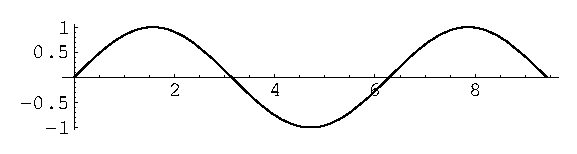
\includegraphics[width=8.5cm]{Figures/image1}}
%%  \vspace{2.0cm}
%  \centerline{(a) Result 1}\medskip
%\end{minipage}
%%
%\begin{minipage}[b]{.48\linewidth}
%  \centering
%  \centerline{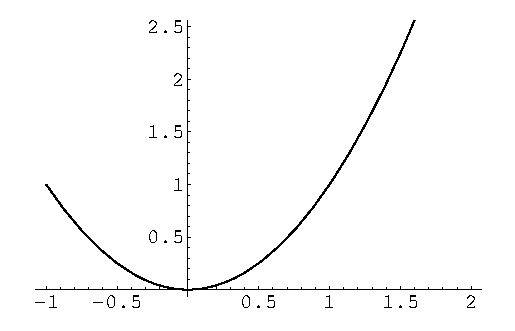
\includegraphics[width=4.0cm]{Figures/image3}}
%%  \vspace{1.5cm}
%  \centerline{(b) Results 3}\medskip
%\end{minipage}
%\hfill
%\begin{minipage}[b]{0.48\linewidth}
%  \centering
%  \centerline{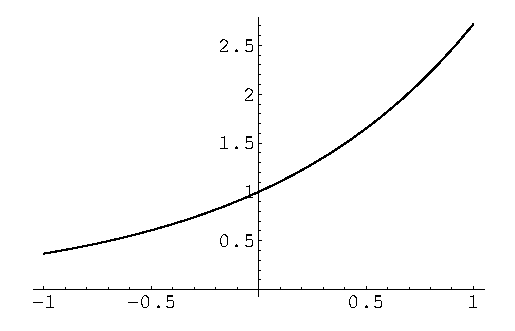
\includegraphics[width=4.0cm]{Figures/image4}}
%%  \vspace{1.5cm}
%  \centerline{(c) Result 4}\medskip
%\end{minipage}
%%
%\caption{Example of placing a figure with experimental results.}
%\label{fig:res}
%%
%\end{figure}


% To start a new column (but not a new page) and help balance the last-page
% column length use \vfill\pagebreak.
% -------------------------------------------------------------------------
\vfill
%\pagebreak

%\section{COPYRIGHT FORMS}
%\label{sec:copyright}
%
%You must include your fully completed, signed IEEE copyright release form when
%form when you submit your paper. We {\bf must} have this form before your paper
%can be published in the proceedings.
%
%\section{REFERENCES}
%\label{sec:ref}

%List and number all bibliographical references at the end of the
%paper. The references can be numbered in alphabetic order or in
%order of appearance in the document. When referring to them in
%the text, type the corresponding reference number in square
%brackets as shown at the end of this sentence \cite{C2}. An
%additional final page (the fifth page, in most cases) is
%allowed, but must contain only references to the prior
%literature.

% References should be produced using the bibtex program from suitable
% BiBTeX files (here: refs). The IEEEbib.bst bibliography
% style file from IEEE produces unsorted bibliography list.
% -------------------------------------------------------------------------

\bibliographystyle{ieeetr}
\bibliography{references_icip14}
\vfill
\end{document}
